% Journal:
%   Journal of Ambient Intelligence and Smart Environments (JAISE), IOS Press
%   Web Intelligence and Agent Systems: An International Journal (wias)
%   Semantic Web: Interoperability, Usability, Applicability (SW)
% Latex 2e
% Test file iosart2c.tex

%[seceqn,secfloat,secthm,crcready]

% options: wias, jaise, sw
\documentclass{iosart2c}

\usepackage{listings}

\usepackage[T1]{fontenc}
\usepackage{times}%

\usepackage{natbib}
%\usepackage[dvips]{hyperref}
\usepackage{amsmath}
\usepackage{dcolumn}
%\usepackage{endnotes}
\usepackage{graphics, url}


\newcolumntype{d}[1]{D{.}{.}{#1}}


\firstpage{1} \lastpage{5} \volume{1} \pubyear{2009}


\begin{document}
\begin{frontmatter}                           % The preamble begins here.

%\pretitle{Pretitle}
\title{Using the LLOD Cloud for Querying Linguistic Resources%\thanks{Footnote in title.}
} % CHANGE AS SUITED - RL.

\runningtitle{Using the LLOD Cloud for Querying Linguistic Resources}
%\subtitle{Subtitle}

%\review{Name Surname, University, Country}{Name Surname, University, Country}{Name Surname, University, Country}

\author[A,B]{\fnms{Richard} \snm{Littauer}},
\author[C]{\fnms{Steven} \snm{Moran}},
%\thanks{Corresponding author. E-mail: editorial@iospress.nl.}%\thanks{Do not use capitals for the author's surname.}
and
\author[D]{\fnms{Boris} \snm{Villazon-Terrazas}}
\runningauthor{Littauer, Moran and Villazon-Terrazas}

%\address[A]{Journal Production Department, IOS Press, Nieuwe Hemweg 6b, 1013 BG, Amsterdam,\\ The Netherlands\\ E-mail: first@somewhere.com}
%\address[B]{Department first, then University or Company name, Insert a complete correspondence (mailing) address, Abbreviate US states, Include country\\ E-mail: \{second,third\}@somewhere.com}

\address[A]{Department of Intelligent Computer Systems, University of Malta, Msida, MSD2080, Malta}
\address[B]{Computational Linguistics Department, Saarland University, Saarbr\"ucken, 66121, Germany\\  E-mail: littauer@coli.uni-saarland.de}
\address[C]{Research Unit Quantitative Language Comparison, Ludwig Maximilian University, Geschwister Scholl Platz 1, D-80539 Munich, Germany\\ 
E-mail: bambooforest@gmail.com} %Steve? Probably not the right email. 
\address[D]{Intelligent Software Components, iSOCO, S.A., Av. del Partenon 16-18, Madrid, Spain\\
E-mail: bvillazon@isoco.com}

\begin{abstract}
The Semantic Web offers a unique opportunity to query for large amount of data which would otherwise exist only in fragmented databases. Recently, the Open Linguistics Working Group has been developing a sub cloud of ontologies which conform to the Linked Open Data paradigm with the intent to enable computational linguists to utilise the Semantic Web. Here, we present a SPARQL endpoint for the Linguistics Linked Open Data cloud. We showcase how to query for language resources within the cloud, with example query results for language resources from multiple databases, which previously would have had to have been collected individually and arduously. It is hoped that the work presented here will expedite use of the Linguistics Linked Open Data cloud by researchers. 

%122 words at present.

%The abstract should be clear, descriptive, self-explanatory and no longer than 200 words. It should also be suitable for publication in abstracting services. Do not include references or formulae in the abstract.
\end{abstract}

\begin{keyword}
Semantic Web\sep Linked Data\sep LLOD\sep Linguistics\sep Typology\sep Language Resources
%Keyword one\sep keyword two\sep keyword three\sep keyword four\sep keyword five
\end{keyword}
\end{frontmatter}

\section{Introduction}
%
%Richard's hackday project aimed at querying the LLOD via ISO 639-3
%code. At that time, these queries worked (see below for several of
%them). Now they don't seem to return anything (hence I haven't
%included them in the MLODE hack day results). There might be some
%fairly obvious reason for them not working, but I'm not sure what it
%is. I do remember that at one point the URL or the endpoint or
%something was changed for some reasons (hosting was with Pablo's
%group?).
%I do think though that the ability to query LLOD for resources via
%language code, etc., is a very, very strong selling point for the data
%post-proceedings and for the LLOD cloud in general. We aren't going to
%get any serious users (do we currently have any users?) beyond the
%Leipzig group (and perhaps some others), if it's not functioning (or
%if we can't explain how to use it since what was once working no
%longer works).
%
%It would be great to get such "exploratory" data queries working and I
%know Richard and a few others want to submit something to the data
%post-proceedings on exactly that.

%ENDPOINT: http://mlode-sparql.nlp2rdf.org/sparql

% The amount of computational linguistic resources available has grown considerably in recent years. This is true of both primary resources -- audio corpora, dictionaries, ontologies -- and secondary resources - parsers, segmenters, WordNets. However, limited interoperability and licensing constraints between primary resources are major obstacles for data use and reuse. Interoperability can be either structural, apparent when similar formalisms are used to access data, or conceptual, where the resources themselves share a common vocabulary \citep{ide-pustejovsky2010-interoperability}. Representing data so that they conform to the paradigms and languages of the Semantic Web fosters interoperability for resources, as well as providing an infrastructure with a vibrant development community that can be used to query these resources.

The amount of linguistic resources available on the Web has grown considerably in recent years. This is true of both data resources, such as lexical data, multimedia recordings and annotated corpora, as well as for computational tools cleaning and analysis, such as chunkers, part of speech taggers and parsers. However, limited interoperability between data formats and data licensing constraints are major obstacles for data use, reuse and sharing. Representing data so that they conform to the Semantic Web framework fosters interoperability of resources, as well as providing an infrastructure with a vibrant development community that can be used to query these resources. Linked Data refers to Semantic Web framework best practices for publishing and connecting structured data. One initiative to share openly available data published in Linked Data is called Linked Open Data.

% Interoperability can be either structural, apparent when similar formalisms are used to access data, or conceptual, where the resources themselves share a common vocabulary \citep{ide-pustejovsky2010-interoperability}. 

The Linguistic Linked Open Data (LLOD) cloud\footnote{\url{http://linguistics.okfn.org/resources/llod/}} is a sub-cloud of the Linked Open Data cloud,\footnote{\url{http://richard.cyganiak.de/2007/10/lod/}} consisting of data from databases of linguistic corpora and metadata that conforms to the Linked Open Data paradigm \citep{bernersLee2006_linkeddata}. This cloud is being developed by the Open Linguistics Working Group (OWLG) \cite{owlg4lrec}, an open community that aims to promote open data in linguistics and that facilitates communication between researchers from different scientific disciplines and communities. The LLOD  contains data from dozens of publicly available online databases that have been converted to RDF. Here, we briefly outline the technologies behind the LLOD (described at length elsewhere, cf. \cite{ldl-llod, ChiarcosLOD}), and, for the first time we discuss accessing data in the LLOD through a SPARQL endpoint set up during the Multilingual Linked Open Data for Enterprises workshop. We provide a couple of examples of how to use the endpoint to query across resources linked in the LLOD. The first query displays all resources within the cloud that have information related to a language-specific ISO 639-3 three letter language name identifier. Once data sources that contain information about a given language are identified, each data source can then be further queried for detailed information regarding that given language. Our second example query identifies the typological features of a given language that are available in the World Atlas of Language Structures (WALS) \citep{Haspelmath_etal2008}. We conclude by briefly discussing the possible applications of querying the LLOD cloud for linguistic analysis and its potential use to language researchers. 


\section{The Semantic Web}
The representation formalisms and technologies that make up the Semantic Web can be used to enable interoperability for language databases on a wide scale. The Linked (Open) Data paradigm \citep{bernersLee2006_linkeddata} sets out four rules for representation of web resources: 
\begin{enumerate}\item Referred entities should be designated by using Uniform Resource Identifiers (URIs),
\item these URIS should be resolvable over HTTP,
\item data should be represented by means of specific W3C standards (such as RDF),
\item and a resource should include links to other resources. \end{enumerate}
These rules facilitate information integration, and thus, interoperability, in that they require that entities can be addressed in a globally unambiguous way (1), that they can be accessed (2) and interpreted (3), and that entities that are associated on a conceptual level are also physically associated with each other (4). \cite{ChiarcosLOD} 


Following these rules, the Resource Description Framework (RDF) was laid down as a language meant to provide metadata for various resources. In RDF, information is expressed in triples (property, subject, and object), and RDF collections of data are represented by URIs, which are globally unambiguous in the web. This way, resources can link to each other, and an valid, coherent ontology can be more easily created. 

SPARQL \cite{prud2008sparql} is a standardised query language for RDF data. Inspired by SQL, SPARQL also uses a triple notation similar to RDF. It not only supports querying data from a single database accessible over HTTP - known as SPARQL endpoints - but also can query multiple databases from a single endpoint. It is this feature which allows the use of massive ontologies to be made out of several databases, creating a cloud of interoperable resources. RDF and SPARQL together are thus the main constituents of the Semantic Web. 


\section{The LLOD cloud}
\begin{figure*}[t!hpb]
\caption{The LLOD Cloud}\label{f1}
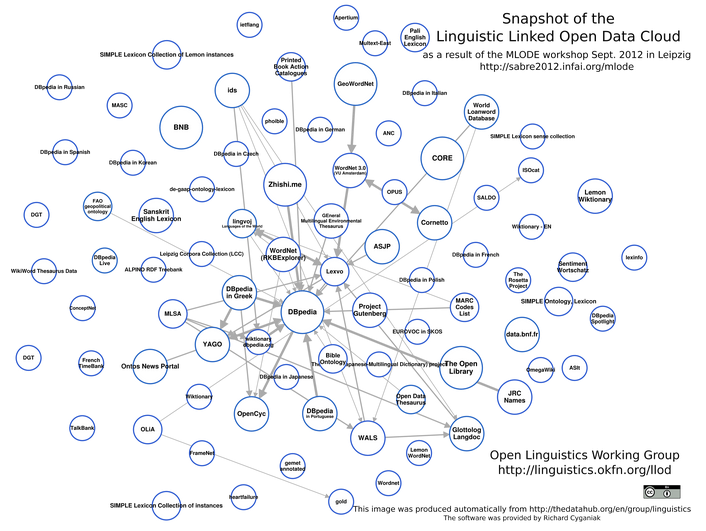
\includegraphics[width=15cm,keepaspectratio]{llod.png}
\end{figure*}

The Linguistics Linked Open Data cloud represents a portion of the Semantic Web network, and is specifically a sub cloud of the Linked Open Data cloud. It is maintained by the Open Linguistics Working Group\footnote{\url{http://linguistics.okfn.org/}}, which has three main goals for promoting openness in Linguistics: \begin{enumerate} \item Promoting the idea of open linguistic resources; \item Developing the means for the representation of open data; \item Encouraging the exchange of ideas across different disciplines. \end{enumerate}

Building an interoperable, linked data cloud is directly in line with these aims. The Open Knowledge Foundation, the umbrella organisation for the OWLG and other working groups, defines `openness' as "A piece of content or data [that] is open if anyone is free to use, reuse, and redistribute it -- subject only, at most, to the requirement to attribute and share-alike."\footnote{\url{http://opendefinition.org}} With this in mind, different databases within the Linked Open Data cloud have been marked out for inclusion within the LLOD. A diagram for the LLOD, developed by Cyganiak and Jentzsch, can be found at \url{http://lod-cloud.net} - this diagram is displayed in Fig. \ref{f1}. 

The following criteria must be met for a new linguistic resource to be included in the LLOD cloud: \begin{enumerate}\item The data is resolvable through HTTP, \item it is provided as RDF, \item it contains links to another data set in the diagram, and \item the entire data set must be available.\end{enumerate}. At the time of writing, the LLOD has {\it draft} status, meaning that several of the resources may point only to resource metadata, although each has been promised to be uploaded and linked to the LLOD in the near future. There are already many resources within the cloud, however, such as DBpedia, different RDF versions of WordNet, Cornetto (Dutch WordNet), OpenCyc, and the Open Data Thesaurus, metadata repositories like Lexvo and lingvoj. GOLD and ISOcat are currently available, although their license conditions are yet to be clarified. 




\section{Querying the LLOD for language resources}
%%
%%Richard Littauer, Didier Cherix and Steven Moran
%%http://mlode.nlp2rdf.org/sparql
%%

\begin{center}
\begin{table*}[t!hbp]
\caption{Query for resources with a given ISO 639-3 code} \label{t1}
\begin{tabular}{lll}
\hline
{\footnotesize \lstinputlisting{query_2}} \\
\hline
\end{tabular}
\end{table*}
\end{center}

\begin{table*}[b!htp]
\caption{Result for query for resources with a given ISO 639-3 code} \label{t2}
\begin{tabular}{lll}
\hline
\url{relation} \\
\url{http://www.llmap.org/maps/by-code/crw.html} \\
\url{http://www.ethnologue.com/show_language.asp?code=crw} \\
\url{http://en.wikipedia.org/wiki/ISO_639:crw} \\
\url{http://www.lexvo.org/data/iso639-3/crw} \\
\url{http://www.sil.org/iso639-3/documentation.asp?id=crw} \\
\url{http://multitree.org/codes/crw} \\
\url{http://scriptsource.org/lang/crw} \\
\url{http://www.language-archives.org/language/crw} \\
\url{http://odin.linguistlist.org/igt_urls.php?lang=crw} \\
\url{http://linguistlist.org/forms/langs/LLDescription.cfm?code=crw} \\
\url{http://www.glottolog.org/resource/languoid/id/chra1242} \\
\hline
\end{tabular}
\end{table*}

A SPARQL endpoint for the LLOD was set up as part of the MLODE conference. This endpoint is located at: \url{http://mlode-sparql.nlp2rdf.org/sparql}. 

In order to test the use of this endpoint, and in order to showcase how the LLOD can be queried and used in a non-theoretical capacity, we present the two queries below. These are by no means the only queries possible on the endpoint, nor do they represent the full nature of the LLOD -- rather, these were judged to be of the most interest to linguistic researchers using online databases already. 

Using the SPARQL endpoint, we set ourselves the goal of devising SPARQL queries to identify all resources in the LLOD cloud that have data with regard to a specific ISO 639-3 unique language name identifier. ISO 639-3 identifiers are maintained by the Summer Institute of Linguistics\footnote{http://www.sil.org/iso639-3/} and consist of three-letter codes that refer to one of the existing 7000~ extant languages in the Ethnologue  database.\footnote{A full list can be found here: \url{http://www.sil.org/iso639-3/download.asp}} This query is given in Table 1. The three-letter language code used is [crw], the language code for Chrau, a Vietnamese language spoken in Southeast Asia. Here, the ISO code is retrieved from the WALS database by querying using the WALS native three-letter identifier [chr]. 

To use the endpoint, go to the link above and paste the query into the `Query Text' box, and press `Run Query'.\footnote{Uncheck the `Default Data Set Name (Graph IRI)' in the top entry box by deleting \url{http://mlode.nlp2rd.org}, so that the box is empty.} The query will then fire. The hyperlink of the loaded query can be used as a way to refer to that result without needing to re-enter the query for each iteration. The output of the query, at the time of writing, is given in Table 2. There are several resources that contain a variety of information on the Chrau language, including details about its geographical location (where speakers of Chrau live), its population, language family information, the system used to write the language, etc. As is clear, there are several datasets already available in the LLOD clod that can be used to gather more, related information about specific information.

Our second example query retrieves all of the information in WALS for a specific ISO 639-3 code. As mentioned above, alongside ISO 639-3 codes, WALS also defines its own language name identifiers because its compilers have a different idea of what the set of mutually unintelligible language varieties are. For this reason, researchers often need to create wrappers to mine data several resources, such as the Ethnologue (the originator of language code), SIL (the gatekeeper of the current ISO 639-3 codes), and typology-specific databases and like WALS. It is of course possible to formulate a query that runs using the ISO 639-3 language code, then finds the WALS code, and then gathers all data from WALS as well as other databases using the original ISO code. The use of this sort of query for mining information about languages, which have various alternative names and even different `standard' codes identifying those name, cannot be understated due to the amount of time and effort it saves the researcher, especially from search multiple different resources. A query that gathers WALS data is given in Table 3. The results of the query are given in Table 4. Here we have limited the results to 3 entries.\footnote{This can be done by appending LIMIT 3 after the closing bracket at the end of the code snippet.}

\begin{table*}
\caption{Query for all information for a given ISO 639-3 code on WALS} \label{t1}
\begin{tabular}{lll}
\hline
{\footnotesize \lstinputlisting{query_1}} \\
\hline
\end{tabular}
\end{table*}


\begin{table*}
\caption{Results (LIMIT 5) for WALS for a given ISO 639-3 code} \label{t1}
\begin{tabular}{p{.5cm}p{4cm}p{2cm}p{2cm}p{.5cm}p{.5cm}p{3.5cm}}
\hline
label & descr &ref & area & lat & long &genus \\
Chrau & The language has no morphologically dedicated second-person imperatives at all&Thomas 1971 & Verbal Categories&10.75&107.5&http://wals.info/genus/bahnaric\\
Chrau &The prohibitive uses the verbal construction of the second singular imperative and a sentential negative strategy not found in (indicative) declaratives&Thomas 1971&Verbal Categories&10.75&107.5&http://wals.info/genus/bahnaric \\
Chrau&Adpositions without person marking&Thomas 1971&Verbal Categories&10.75&107.5&http://wals.info/genus/bahnaric \\
\hline
\end{tabular}
\end{table*}





\section{Conclusions}
The queries presented here are a small subset of the possibilities of the LLOD cloud. As more databases are added, more informational will be able to bee retrieved that can be used in linguistic research or for commercial uses. 

%FILL IN MORE. 


\bibliographystyle{IEEEtran} %Probably not the style we should use???
\bibliography{bib.bib}

\end{document}
